\documentclass[12pt]{article}[abntex2]
\usepackage[brazil]{babel}
\usepackage{graphicx} % Required for inserting images
\usepackage{sbc-template}
\usepackage{indentfirst}
\usepackage[alf]{abntex2cite}
\usepackage{multicol}
\usepackage{adjustbox}
\usepackage{tabularray}
\usepackage{ragged2e}

\newcommand{\D}{\displaystyle}

\title{Seleção, pontuação e ranqueamento de provedores Serverless utilizando métodos de Decisão Multicritério}
\author{Leandro Ribeiro Rittes, Adriano Fiorese}

\address{Programa \\ 
Universidade do Estado de Santa Catarina
  (UDESC)\\
  Joinville, Santa Catarina, Brasil 89219-710
  \email{leandro.rittes1990@edu.udesc.br, adriano.fiorese@udesc.br}
}

\begin{document}

\maketitle

\section{INTRODUÇÃO}
Conforme a tecnologia avança, torna-se cada vez mais desafiador identificar a melhor abordagem ou método para desenvolver um software que atenda aos objetivos finais sem se tornar economicamente inviável e tecnicamente complexo. A vasta área de desenvolvimento de software, incluindo front-end, back-end, DevOps, infraestrutura, entre outras, oferece centenas de tecnologias diferentes. Essa dificuldade da escolha da tecnologia ideal pode proporcionar o melhor desempenho ao software tanto em custo, complexidade, manutenção, etc.

Especificamente na área de infraestrutura, existem diversas tecnologias possíveis, algumas até redundantes. A escolha da tecnologia adequada pode ser influenciada pela disponibilidade de mão de obra especializada, que em alguns momentos do mercado, pode ser escassa e, portanto, economicamente inviável. Um setor de uma empresa que pode ter um dos maiores custos é o de infraestrutura, pois a contratação de profissionais qualificados e a manutenção de servidores operando 24 horas por dia, 7 dias por semana, são despesas elevadas. 

A terceirização dos serviços de infraestrutura, conhecida como serverless, representa uma estratégia eficaz para enfrentar diversos desafios. Essa abordagem foca na disponibilização de servidores por grandes empresas ao mercado, resultando em uma redução significativa dos custos de manutenção para tais empresas. Isso ocorre porque os custos associados à manutenção dos servidores seriam mantidos independentemente da sua utilização ou não. Para pequenas empresas, isso significa que elas podem se concentrar unicamente na mão de obra necessária para o desenvolvimento de seus softwares, sem preocupações adicionais com a gestão de infraestruturas físicas. Assim, elas só precisam arcar com o aluguel dos servidores necessários para suas operações. Ao optar pela contratação de uma empresa que oferece serviço serverless, as empresas contratantes podem externalizar os custos e responsabilidades relacionadas à manutenção e operação desses recursos, liberando assim tempo e recursos para focar no desenvolvimento de software. Esta estratégia não apenas economiza dinheiro, mas também promove maior eficiência e qualidade no produto final, graças à capacidade da equipe interna de se dedicar integralmente ao seu trabalho.

Reconhecendo a relevância de optar por uma solução de infraestrutura de terceiros, este estudo visa analisar e escolher técnicas de decisão multicritério para selecionar, avaliar e classificar provedores de serviços serverless. Esta analise auxiliará os usuários a comparar vários fornecedores mediante diversos critérios importantes, simplificando a adoção de decisões fundamentadas sobre a escolha do provedor que melhor atende às suas necessidades específicas. A estrutura deste artigo é organizada da seguinte maneira: introdução, Referencial Teórico, Trabalhos relacionados, metodologia de pesquisa, apresentação e análise dos dados, e considerações finais.

% Pergunta de pesquisa: Qual é o mais adequado provedor serverless para os clientes…

\section{REFERENCIAL TEÓRICO}
% ETAPA1: Referencial teorico do que? Quais os conceitos que precisam ser definidos no trabalho
\subsection{Serverless}
Serverless, ou computação sem servidor, é um paradigma de desenvolvimento que permite aos desenvolvedores criar e executar aplicações sem a necessidade de gerenciar servidores ou infraestrutura de backend e como dito por Castro \cite{castro2019}, em 2020 os gastos com infraestrutura e software baseados em tecnologia na nuvem por empresas de TI já poderiam chegar a 67\%. Embora os servidores ainda sejam utilizados, eles são abstraídos do processo de desenvolvimento, e um pensamento compartilhado por Castro \cite{castro2019} e Wen \cite{wen2023rise} e por muitos na área, é que esse novo paradigma de desenvolvimento permite que os desenvolvedores se concentrem exclusivamente na lógica de negócios e no código da aplicação. O provedor de nuvem assume a responsabilidade pelo provisionamento, manutenção e escala da infraestrutura, oferecendo uma experiência de desenvolvimento mais eficiente e econômica, Vieira \cite{gomes_computacao_2020} explica que uma das principais característica do serverless é a escalabilidade\\

\begin{flushright}
\begin{minipage}{10cm}
\fontsize{11}{12}\selectfont
em momentos nos quais houver muitos eventos para serem processados, mais funções podem ser invocadas mais rápido e a um custo tanto financeiro quanto computacional potencialmente menor do que ativar mais máquinas virtuais ou contêineres.
\end{minipage}
\end{flushright}

Como é citado na fala de Vieira \cite{gomes_computacao_2020} este modelo é caracterizado pela execução sob demanda, onde os recursos computacionais são escalados automaticamente conforme necessário, e os custos são baseados apenas nos recursos utilizados durante a execução do código. Isso significa que não há cobrança por capacidade inativa, resultando em economia significativa para as empresas.

Atualmente, todos os principais provedores de serviços em nuvem oferecem so\-luções serverless, incluindo AWS Lambda da Amazon, Azure Functions da Microsoft, Google Cloud Functions do Google e IBM Cloud Code Engine da IBM. Essas plataformas permitem que os desenvolvedores aproveitem os benefícios da computação sem servidor, facilitando a criação de aplicações nativas de nuvem escaláveis e eficientes.

A solução serverless representa uma evolução significativa na forma como as aplicações são desenvolvidas e executadas, oferecendo uma abordagem mais eficiente e econômica para o gerenciamento de infraestrutura. Ao permitir que os desenvolvedores se concentrem na lógica de negócios e no código da aplicação, enquanto delegam a gestão da infraestrutura aos provedores de nuvem, o serverless está transformando a maneira como as empresas operam e inovam no mundo digital.


\subsection{Decisão Multicritério}
O Método de Análise Multicritério de Decisão (AMD) do inglês Multi-criteria decision analysis (MCDA), é uma abordagem que vem ganhando destaque no campo da tomada de decisões complexas. Este método é particularmente útil em situações onde não basta considerar apenas um único critério para tomar uma decisão, mas sim múltiplos aspectos que podem ser conflitantes entre si. A aplicação do MCDA abrange diversas áreas, desde engenharia e gestão até meio ambiente, políticas públicas e saúde, demonstrando sua versatilidade e utilidade prática.

As vantagens do uso do MCDA são evidentes. Ele permite a consideração de múltiplos critérios, mesmo aqueles qualitativos ou intangíveis, fornecendo um processo de decisão transparente e auditável. Isso facilita a comunicação entre os tomadores de decisão e promove a tomada de decisões coerentes e embasadas em critérios objetivos.

No entanto, é importante reconhecer que o uso do MCDA também apresenta desafios. A aplicação do método pode ser complexa, exigindo conhecimento técnico especializado e tempo para coleta e análise de dados. A definição dos pesos para os diferentes critérios pode ser influenciada por valores pessoais ou visões de mundo dos decisores, introduzindo um elemento de subjetividade no processo. Além disso, nem todos os critérios podem ser facilmente quantificados, o que pode complicar a comparação entre alternativas. E, finalmente, o processo de decisão multicritério pode ser demorado, especialmente quando envolve um grande número de alternativas ou critérios.

Apesar desses desafios, o valor do MCDA reside em sua capacidade de fornecer uma estrutura organizada para avaliar e comparar alternativas de forma transparente e sistemática. Ao permitir a consideração de múltiplos critérios, promover a transparência e encorajar a participação das partes interessadas, o MCDA facilita a tomada de decisões mais informadas, equilibradas e sustentáveis.

No âmbito do MCDA, a diversidade de abordagens disponíveis é vasta, cada uma adequada a diferentes tipos de problemas. Portanto, a seleção cuidadosa do método mais apropriado torna-se crucial. Este artigo concentra-se especificamente na tarefa de selecionar, pontuar e ranquear provedores serverless a partir de critérios específicos. Com base nessa necessidade, os métodos escolhidos foram o Analytic Hierarchy Process (AHP), PROMETHEE e TOPSIS, conforme destacado na tabela de Ishizaka.\cite{Multi_criteria_2013}.

\subsubsection{Analytic Hierarchy Process (AHP)}
O Analytic Hierarchy Process (AHP), concebido por Thomas L. Saaty na década de 1970, surgi como uma metodologia para auxiliar na tomada de decisões complexas. Este método, que se destaca pela sua capacidade de decompor problemas intricados em componentes gerenciáveis através de uma hierarquia bem definida, oferece uma abordagem sistemática para avaliar e comparar múltiplos critérios e alternativas. Ao empregar comparações pareadas, o AHP não só facilita a determinação da importância relativa de cada critério e alternativa, mas também calcula um peso ou prioridade para cada um deles, auxiliando para a escolha mais adequada.

Contudo, como toda ferramenta, o AHP não está imune a desafios. A subjetividade inerente às comparações pareadas, a potencial complexidade na gestão de problemas de grande escala e a sensibilidade dos resultados às mudanças nos pesos atribuídos aos critérios são aspectos que devem ser cuidadosamente considerados. Adicionalmente, a implementação efetiva do AHP pode demandar um certo grau de conhecimento especializado, destacando a importância de uma compreensão profunda dos princípios subjacentes ao método.

Dado esse panorama sobre o método AHP, a tabela construída por AYALA e FRANK \cite{ayala2013metodos} a seguir apresenta as vantagens e desvantagens da utilização do método AHP

\begin{center}
\textbf{\Large{Vantagens}}\\
\end{center}
\begin{multicols}{2}
        \begin{itemize} 
\item A grande difusão do AHP deve-se
        principalmente a sua simplicidade,
        facilidade de utilização y grande
        flexibilidade devido a que pode ser
        integrado com outras técnicas, como por
        exemplo, o QFD e a matriz SWOT. Além
        disso, a utilização do método proporciona
        uma grande confiabilidade e aceitação
        devido a seu aprofundado estudo na
        literatura e sua ampla aplicação e
        avaliação nas diferentes áreas \cite{RODRÍGUEZ2008toma,norris1995ius}
        \item Uma grande força do AHP é a
        possibilidade de medição da consistência
        interna dos julgamentos dos stakeholders.
        Ainda, a obrigatoriedade de interação entre
        o analista e o decisor pode-se observar
        como uma vantagem, já que permite que
        todos os envolvidos entendam o problema
        da mesma forma. Por sua vez, a síntese
        dos resultados permite a comparação das
        prioridades e importância relativa de cada
        fator \cite{VilasAnalise,liberatore1997group,salomon1999justificativas,boucher1997comparison,wang2008fuzzy,norris1995ius}
        \end{itemize} 
        \end{multicols}

\newpage
\begin{center}
\textbf{\Large{Desvantagens}}\\
\end{center}
\begin{multicols}{2}
        \begin{itemize} 
        \item O AHP tem um limite máximo aconselhado
        de VILAS, 2008 elementos de comparação, já
        que o número de julgamentos par a par
        incrementa-se a razão de (n(n-1)/2) e muitas
        comparações tornam o trabalho difícil e tedioso
        perdendo sua confiabilidade. \cite{salomon1999justificativas,morita1999modelos,gomes2003conceitos,guglielmetti2003comparaccao}
        \item É preciso montar uma estrutura hierárquica
        em cada nível com atributos totalmente
        independentes entre ele, situação que pode não
        ocorrer em alguns casos. \cite{liu2008access,saaty2013analytic}
        \item Os pesos obtidos da comparação par a par
        são fortemente criticados por não refletir as
        reais preferências das pessoas. \cite{linkov2008appendix}
        \item A escala do AHP não permite expressar um
        grau de incerteza respeito ás comparações e
        alternativas incomparáveis não são permitidas.
        Além disso, a necessidade de consenso para a
        determinação dos pesos e prioridades, também
        pode verse como uma desvantagem já que pode
        levar a que líderes influentes distorçam a
        opinião do resto da equipe. \cite{kangas2005multiple, VilasAnalise}
        \item Uma das maiores críticas ao AHP é respeito
        ao rank reversal que pode causar sérios
        problemas, devido a que quando uma nova
        alternativa é introduzida num problema de
        decisão, pode mudar radicalmente o ranking
        previamente estabelecido. \cite{kangas2005multiple,boucher1997comparison}
        \item Outra área onde o AHP está sendo criticado
        é na maneira em que ele extrai e estima os
        pesos dos critérios. Ao mesmo tempo, outra
        limitação é a necessidade de ter
        obrigatoriamente duas alternativas para poder
        aplicar o método, o que faz o método
        inadequado para avaliar situações onde se
        precisa saber o comportamento de uma única
        alternativa. \cite{boucher1997comparison}
        \end{itemize} 
\end{multicols}

Em suma, o Analytic Hierarchy Process representa uma abordagem robusta e estruturada para a tomada de decisões em ambientes caracterizados pela presença de múltiplos critérios. Ao proporcionar uma base quantitativa sólida, facilitando a análise comparativa e promovendo a participação inclusiva, o AHP se estabelece como um recurso indispensável para aqueles comprometidos em alcançar decisões informadas, equilibradas e sustentáveis.

\subsubsection{Preference Ranking Organization Method for Enrichment Evaluation (PROMETHEE)}
\subsubsection{Technique for Order of Preference by Similarity to Ideal Solution (TOPSIS)}

\section{TRABALHOS RELACIONADOS}
\section{METODOLOGIA DE PESQUISA}
Este artigo tem como objetivo comparar e avaliar diferentes métodos de Decisão Multicritério (MCDA) aplicados à seleção, pontuação e ranqueamento de provedores de serviços serverless. A pesquisa, de natureza documental e quantitativa, envolveu uma análise aprofundada das informações disponíveis nos sites oficiais dos principais provedores serverless e em relatórios de benchmarking de 2023. O estudo busca identificar o método MCDA mais adequado para a seleção de provedores serverless, considerando um conjunto de critérios relevantes para o mercado. A seção tem como objetivo discutir e apresentar os cálculos, os critérios e o desenvolvimento dos métodos para seleção, pontuação e ranqueamento dos provedores.

\subsection{Critérios de Avaliação}
A seleção e a classificação dos provedores serverless, neste trabalho, foram realizadas por meio de métodos MCDA que se baseiam em um conjunto de critérios ou Indicadores de Desempenho (KPIs). Estes indicadores são fundamentais, pois servem como parâmetros para as avaliações quantitativas e qualitativas, permitindo a comparação e a pontuação das diferentes alternativas. A tabela a baixo apresenta um conjunto de KPIs de um problema fictício para seleção de um computador.

\begin{table}[ht]
\centering
\begin{adjustbox}{width=0.3\textwidth}
\small
\begin{tabular}{|c|c|}
   \hline
   KPIs  & Tipo \\
   \hline
   RAM  &  HB \\
   Core  & NB \\
   Disco & HB \\
   Custo & LB \\
   \hline
\end{tabular}
\end{adjustbox}
\caption{Nomeclatura e tipo de cada PI}
\label{tablePI}
\end{table} 

Para selecionar o melhor computador é preciso saber qual a quantidade de memoria RAM miníma? qual a quantidade exata de core? qual o tamanho de espaço de armazenamento em disco miníma? qual o custo máximo?\\
Conhecendo os principais fatores para a escolha de um computador foi construído a tabela \ref{tablePI} onde na primeira coluna indica a nomenclatura dos KPIs para o computador e na segunda coluna o tipo. No artigo de Moraes \cite{Borges_Fiorese_2018} é abordado e apresentado o tema dos tipos.\\
\begin{quote}
\fontsize{11}{12}\selectfont
    Podemos classificar as PI’s de acordo com a sua função e utilidade, isso quer dizer o quão útil a PI se torna quando os seus valores aumentam ou decaem, e há 3 possibilidades para isso.
\begin{itemize}
    \item \textbf{HB (Higher is Better):} usuários e gestores de sistemas preferem valores maiores em certos indicadores, por exemplo, taxa de transferência do sistema, quantidade de recurso (dinheiro, memória, material, etc), disponibilidade do sistema, etc,  
    \item \textbf{LB (Lower is Better):} usuários e gestores de sistemas preferem valores menores em certos indicadores, por exemplo, tempo de resposta, custo, latência, etc.  
    \item  \textbf{NB (Nominal is Best):} usuários e gestores de sistemas preferem valores específicos, nem alto nem baixo, por exemplo, carregamento para utilização do sistema, uma utilização alto do sistema pode gerar um tempo de resposta alto, em contra partida uma utilização baixa quer dizer que estão usando pouco o sistema.
\end{itemize}
\end{quote}
%\hspace{4cm} {}
Analisando a coluna "tipo" da Tabela \ref{tablePI}, observamos que as PIs "RAM" e "Disco" são diretamente proporcionais à pontuação (quanto maior o valor, maior a pontuação), enquanto a PI "Custo" é inversamente proporcional (quanto menor o valor, maior a pontuação). A PI "Core" receberá a pontuação máxima apenas se corresponder ao valor desejado pelo usuário. Essas informações são cruciais, pois os métodos utilizados neste estudo atribuem pesos diferentes aos critérios, permitindo que o software diferencie entre atributos desejáveis em níveis altos ou baixos.

% Dados
\subsection{Dados}
A coleta de dados foi realizada em duas etapas. Primeiramente, acessamos diretamente os sites oficiais dos principais provedores serverless (AWS Lambda, Google Cloud Functions e Microsoft Azure) em 22/01/2024, para obter os dados mais recentes sobre os serviços oferecidos. Em seguida, complementamos a análise com dados de benchmark provenientes do relatório de Rifai \cite{benchmarkMooner}, que apresenta uma avaliação detalhada de diversos aspectos relevantes para a escolha de um provedor serverless.
Os dados extraídos nos sites oficiais e no relatório, foram utilizados como critérios para os métodos MCDA, abaixo é feito sua descrição.
\begin{itemize}
    \item \textbf{Tempo de computação}: se refere ao Tempo de execução\footnote{Tempo de execução é o resultado da quantidade de requisições multiplicado pela duração da execução (segundos)} (segundos) multiplicado pelo Consumo de recurso convertido em GBs, o resultado é o valor de graça por mês que o usuário pode utilizar. Contabilizado em GB/segundo.
    \item \textbf{1GB/segundo adicional}: valor adicional para 1GB/segundo que o usuário necessitar no tempo de computação que passar da quantidade de graça disponibilizada. Contabilizado em R\$.
    \item \textbf{Arredondamento da Duração}: se refere ao valor inteiro mais próximo será utilizado quando a duração passar do valor pré definido pelo provedor. Contabilizado em milissegundo.
    \item \textbf{Requisição}: se refere a quantidade de requisição de graça por mês o provedor oferece aos usuários.
    \item \textbf{Requisição adicional}: se refere ao valor adicional para cada 1 milhão de requisição que passar da quantidade de requisição de graça por mês. Contabilizado em R\$. 
    \item \textbf{Scalability}: se refere à capacidade do provedor de se ajustar automaticamente para lidar com um aumento ou diminuição na demanda. Contabilizado em binário.
    \item \textbf{Concurrency}:  se refere à capacidade de executar múltiplas instâncias de uma função simultaneamente. Contabilizado em binário.
    \item \textbf{Cold Start}: se refere ao tempo adicional para responder a uma solicitação em uma instância inativa\footnote{Instância inativa é uma instância que executou uma função e foi destruida.}. Contabilizado em segundo.
    \item \textbf{Memory}: se refere a quantidade de memória que o provedor oferece aos usuários para sua aplicação. Contabilizado em MB.
    \item \textbf{Execution Time}: se refere ao tempo máximo que uma função ficará executando uma função. Contabilizado em minuto.
\end{itemize}

% Requisição
\subsection{Requisição}
A requisição do usuário representa a formalização das suas preferências em relação aos critérios de decisão. Através dela, o método MCDA recebe as informações necessárias para construir as matrizes de decisão, realizar os cálculos e gerar um resultado que reflita a hierarquia de preferência do usuário entre as alternativas. Abaixo é demonstrado a forma de uma requisição.

\begin{table}[htbp]
\centering
\begin{tblr}{
    colspec = {
        |Q[l, wd=6cm] |Q[c, wd=3cm] |Q[c, wd=2cm]|
    }, 
    cell{1}{1-3} = {c, cmd=\textbf},
    width=\linewidth,
}
\hline
    PI & Valor & Peso \\
\hline
Tempo de computação  & 400.000 GB/s & 1 \\
1GB/segundo adicional & 0,25 R\$ & 5\\
Arredondamento da Duração & 1 ms & 1\\
Requisição & 1000 & 9\\
Requisição adicional & 0,5 R\$ & 7\\
Scalabilidade & 1 & 9\\
Concorrência & 1 & 9\\
Cold Start & 1 & 9\\
Memória & 512 MB & 5\\
Tempo de Execução & 30 min & 9\\
\hline
\end{tblr}
\caption{Formato de uma requisição}
\label{tab:requisicao}
\end{table}

Os pesos atribuídos a cada Indicador de Desempenho (PI) refletem a importância relativa de cada critério na decisão do usuário. Utilizando uma escala de 1 a 9, o algoritmo calcula a pontuação final dos provedores, priorizando aqueles que melhor atendem às preferências do usuário.
A escolha da escala de 1 a 9 se deu ao fato dos métodos MCDA já os utilizarem e é uma forma melhor entendida pelo usuário. 
\newpage

\begin{table}[ht]
\centering
\begin{adjustbox}{width=0.7\textwidth}
\small
\begin{tabular}{|c|l|}
\hline
\textbf{Peso} & \textbf{Importância} \\
\hline
1 & Sem Importância \\
2 & Importância Muito Baixa \\
3 & Importância Baixa \\
4 & Importância Moderada \\
5 & Importância Média \\
6 & Importância Relativamente Alta \\
7 & Importância Alta \\
8 & Importância Muito Alta \\
9 & Importância Máxima \\
\hline
\end{tabular}
\end{adjustbox}
\caption{Valor e nomeclatura do peso}
\label{tab:peso}
\end{table} 

% AHP
\subsection{Algoritmo AHP}
A fim de realizar a análise multicritério, optou-se pela utilização da biblioteca python PyDecision, que disponibiliza uma vasta coleção de métodos MCDA, entre eles os métodos empregados neste estudo AHP, PROMETHEE, e TOPSIS. Paralelamente, desenvolvemos uma implementação customizada do algoritmo AHP para fins de comparação. Para avaliar o desempenho das diferentes implementações, foram criados 5 cenários hipotéticos, cada um composto por 1 requisição e por 5 provedores serverless com valores predefinidos e classificação conhecida, dessa forma sabemos o rank do melhor ao pior provedor para cada requisição e podemos avaliar cada implementação. Essa abordagem permitiu comparar a acurácia, o tempo de execução e a capacidade de escalabilidade das diferentes soluções em um ambiente controlado.
Como apresentado na tabela \ref{tab:requisicao} a representação gráfica da requisição nos ajuda a ilustrar ao leitor o input do algoritmo. Cada cenário foi construído com o objetivo de simular uma situação real de seleção de provedor serverless. Em cada cenário foi escolhido 3 PI's com importância máxima (9) e todo o restante com "sem importância" (1). Dessa forma, foi possível avaliar a capacidade do algoritmo MCDA em ranquear corretamente os provedores que melhor atende aos critérios estabelecidos pela requisição.

\newpage
\begin{table}[htbp]
\centering
\begin{tblr}{
    colspec = {
        |Q[l, wd=6cm] |Q[c, wd=3cm] |Q[c, wd=2cm]|
    }, 
    cell{1}{1-3} = {c, cmd=\textbf},
    width=\linewidth,
}
\hline
    PI & Valor & Peso \\
\hline
Tempo de computação  & 400.000 GB/s & 1 \\
1GB/segundo adicional & 0,25 R\$ & 1\\
Arredondamento da Duração & 1 ms & 1\\
Requisição & 1000 & 9\\
Requisição adicional & 0,5 R\$ & 1\\
Scalabilidade & 1 & 1\\
Concorrência & 1 & 1\\
Cold Start & 1ms & 9\\
Memória & 512 MB & 1\\
Tempo de Execução & 30 min & 9\\
\hline
\end{tblr}
\caption{Ilustração de uma requisição criada para teste}
\label{tab:requisicaoTest}
\end{table}

Cada cenário consiste em uma única requisição e cinco provedores fictícios, cujos valores foram atribuídos de forma a gerar um ranking predefinido. Para a escolha do provedor ranqueado com a melhor pontuação foi atribuído a ele os 3 PI's com valor de importância máxima (9) e todos os valores esperados pela requisição.

\begin{center}
\textbf{Provedor 1}
\end{center}
\begin{table}[htbp]
\centering
\begin{tblr}{
    colspec = {
        |Q[l, wd=6cm] |Q[c, wd=3cm] |Q[c, wd=2cm]|
    }, 
    cell{1}{1-3} = {c, cmd=\textbf},
    width=\linewidth,
}
\hline
    PI & Valor & Peso \\
\hline
Tempo de computação  & 400.000 GB/s & 1 \\
1GB/segundo adicional & 0,25 R\$ & 1\\
Arredondamento da Duração & 1 ms & 1\\
Requisição & 1000 & 9\\
Requisição adicional & 0,5 R\$ & 1\\
Scalabilidade & 1 & 1\\
Concorrência & 1 & 1\\
Cold Start & 1ms & 9\\
Memória & 512 MB & 1\\
Tempo de Execução & 30 min & 9\\
\hline
\end{tblr}
\caption{\textbf{Provedor com os 3 melhores PI's}}
\label{tab:provedor1}
\end{table}

\newpage
O provedor escolhido para ser a segunda melhor opção obtém o valor esperado de 2 dos 3 PI's com notas máximas e o valor do terceiro critério com nota máxima recebe um valor abaixo ou acima do esperado dependendo do tipo (tabela \ref{tablePI}) e o restante dos critérios recebem valores com nota de importância 1.  

\begin{center}
\textbf{Provedor 2}
\end{center}
\begin{table}[htbp]
\centering
\begin{tblr}{
    colspec = {
        |Q[l, wd=6cm] |Q[c, wd=3cm] |Q[c, wd=2cm]|
    }, 
    cell{1}{1-3} = {c, cmd=\textbf},
    width=\linewidth,
}
\hline
    PI & Valor & Peso \\
\hline
Tempo de computação  & 400.000 GB/s & 1 \\
1GB/segundo adicional & 0,25 R\$ & 1\\
Arredondamento da Duração & 1 ms & 1\\
Requisição & 1000 & 9\\
Requisição adicional & 0,5 R\$ & 1\\
Scalabilidade & 1 & 1\\
Concorrência & 1 & 1\\
Cold Start & 1ms & 1\\
Memória & 512 MB & 1\\
Tempo de Execução & 30 min & 9\\
\hline
\end{tblr}
\caption{\textbf{Provedor com os 2 melhores PI's}}
\label{tab:provedor2}
\end{table}

Sendo assim o provedor ranqueado como terceiro melhor obtém 1 dos 3 melhores PI's, e os ranqueados como quarto e quinta não obtém nenhum dos 3 melhores e são ranqueados por ordem alfabética.

Dessa forma o rank final é esperado conforme a abaixo:

\begin{center}
\textbf{Ranqueamento}
\end{center}
\begin{table}[htbp]
\centering
\begin{tblr}{
    colspec = {
        |Q[c, wd=2cm] |Q[c, wd=3cm] |
    }, 
    cell{1}{1-2} = {c, cmd=\textbf},
    width=\linewidth,
}
\hline
    Posição & Provedor \\
\hline
1 & Provedor 1 \\
2 & Provedor 2 \\
3 & Provedor 3 \\
4 & Provedor 4 \\
5 & Provedor 5 \\
\hline
\end{tblr}
\caption{\textbf{Rank de provedores fictícios}}
\label{rankTest}
\end{table}


\subsubsection{Cálculo do algoritmo Implementado}
Para ilustrar os cálculos do algoritmo iremos utilizar o problema já abordado de se comprar um computador que melhor atenda o usuário, na figura \ref{fig:problemComp} é ilustrado o objetivo a ser solucionado (escolher o melhor computador), os critérios e seus respectivos valores e as alternativas com seus respectivos valores.

\begin{figure}[!h]
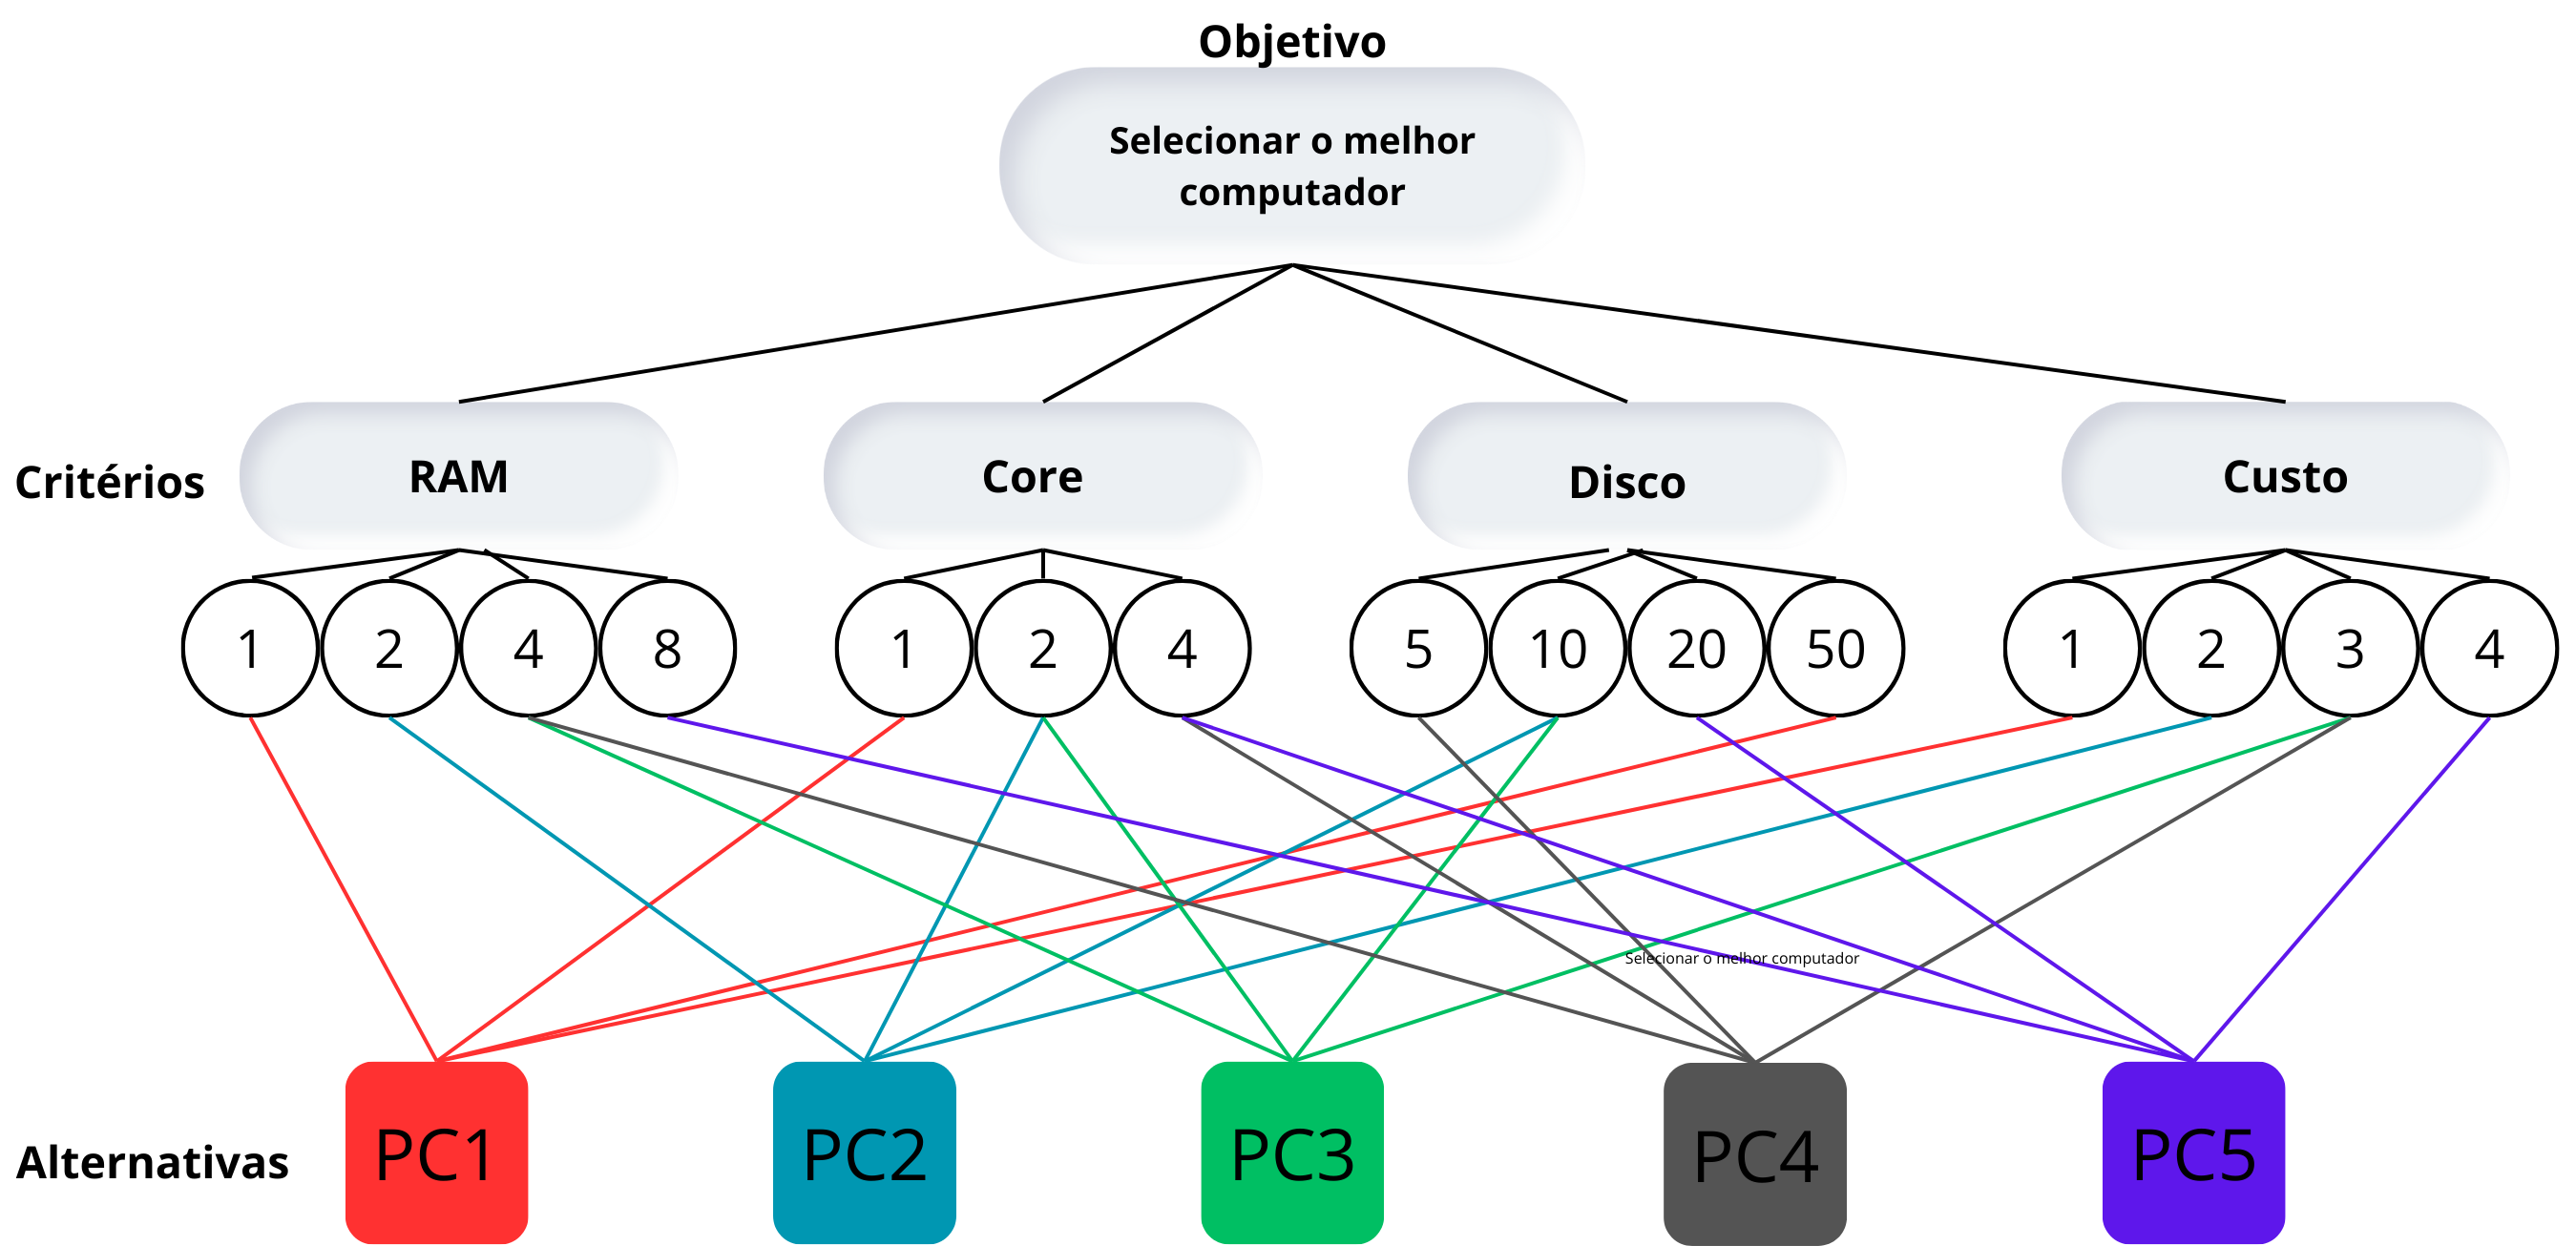
\includegraphics[scale=0.22]{assets/problem}
\caption{Ilustração do problema de selecionar um computador}
\label{fig:problemComp}
\end{figure}

 A tabela \ref{tab:valoresPIComp} é ilustrados os dados de cada PI, sua nomeclatura, seus tipos e todos os valores possiveis.

\begin{table}[ht]
\centering
\begin{adjustbox}{width=0.5\textwidth}
\small
\begin{tabular}{|c|c|l|}
   \hline
   KPIs  & Tipo & Valores \\
   \hline
   RAM  &  HB & 1, 2, 4, 8 \\
   Core  & NB & 1, 2, 4\\
   Disco & HB & 5, 10, 20, 50\\
   Custo & LB & 1, 2, 3, 4 \\
   \hline
\end{tabular}
\end{adjustbox}
\caption{Descrição de PI's do problema de selecionar um computador}
\label{tab:valoresPIComp}
\end{table} 

 A tabela \ref{tab:reqComp} é demonstrado a requisição que será o input do algoritmo para esse problema, contendo as PI's, seus valores desejados e seus pesos (importância).

\newpage
\begin{table}[ht]
\centering
\begin{adjustbox}{width=0.5\textwidth}
\small
\begin{tabular}{|c|c|c|}
   \hline
   PIs  & Valor & Peso \\
   \hline
   RAM  &  2 & 1 \\
   Core  & 2 & 1 \\
   Disco & 40 & 9 \\
   Custo & 2 & 3 \\
   \hline
\end{tabular}
\end{adjustbox}
\caption{Requisição do problema de selecionar um computador}
\label{tab:reqComp}
\end{table} 

Com a requisição (tabela \ref{tab:reqComp}) sendo o input do algoritmo e as 5 alternativas (ilustrada na figura \ref{fig:problemComp}) definidos o primeiro passo do algoritmo é construir a matriz de julgamento demonstrado abaixo.

\begin{figure}[!ht]
\centering
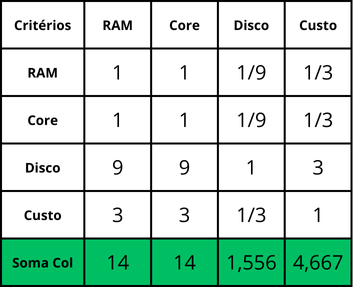
\includegraphics[scale=1]{assets/matJulgPI.png}
\caption{Tabela matriz de julgamento de PI}
\label{tab:matJulgPI}
\end{figure}

A matriz de julgamento das PI's é construída com base nos pesos definido pelo usuário, onde cada célula da matriz é definido o valor da paridade entre o critério da linha sobre o critério da coluna, como podemos ver o critério "Disco" na tabela \ref{tab:matJulgPI} tem peso 9 e o critério "RAM" peso 1, logo na célula da linha "Disco" e coluna "RAM" será o valor 9 e na célula da linha "RAM" e coluna "Disco" será o valor $\D\frac{1}{9}$.
A ultima linha da figura \ref{tab:matJulgPI} é a soma da coluna pois o próximo passo é a normalização dos valores de cada célula, na figura \ref{fig:matJulgPINorm} é ilustrado a tabela normalizada.

\newpage
\begin{figure}[!ht]
\centering
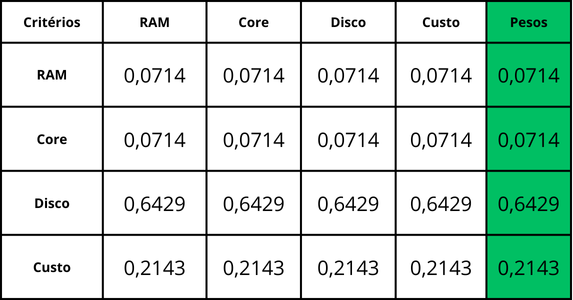
\includegraphics[scale=0.95]{assets/matjulgPINorm.png}
\caption{Tabela matriz de julgamento de PI normalizada}
\label{fig:matJulgPINorm}
\end{figure}

A coluna "Pesos" na figura \ref{fig:matJulgPINorm} corresponde a importância daquele critério em frente aos seus pares, seu valor foi obtido pela soma dos valores da linha divido pela quantidade de valores da coluna, ou seja, a média desses valores.

Após a construção da matriz de julgamento para os critérios, procede-se à constru\-ção de matrizes individuais para cada critério, considerando os valores e pesos definidos na requisição. A Figura \ref{tab:matJulgRAM} ilustra a matriz de julgamento para o critério 'RAM'. As linhas e colunas dessa matriz representam os possíveis valores para 'RAM'. A pontuação atribuída a cada célula depende do valor mínimo de RAM especificado na requisição e da natureza do critério (HB, LB ou NB, conforme Tabela \ref{tablePI}). Por exemplo, para um critério 'HB', valores inferiores ao mínimo especificado recebem a menor pontuação (1), enquanto valores superiores recebem uma pontuação intermediária (5), penalizando excessos que possam implicar em custos adicionais ou outras desvantagens. Caso seja "NB" só receberá o valor máximo caso corresponda ao valor esperado pela requisição, caso contrario receberá o valor 1.


\begin{figure}[!ht]
\centering
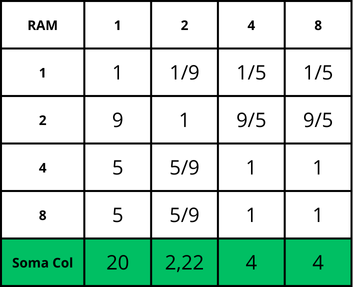
\includegraphics[scale=1]{assets/matJulgRAM.png}
\caption{Tabela matriz de julgamento de RAM}
\label{tab:matJulgRAM}
\end{figure}
\newpage
\begin{figure}[!ht]
\centering
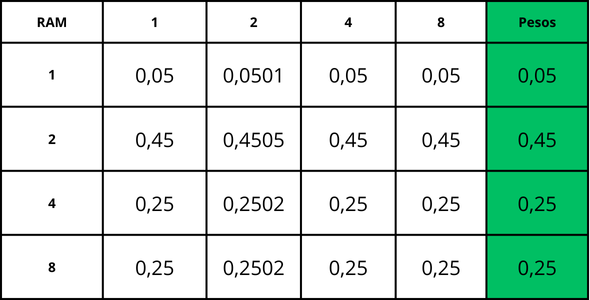
\includegraphics[scale=0.95]{assets/matJulgRAMNorm.png}
\caption{Tabela matriz de julgamento de RAM normalizada}
\label{fig:matJulgRAMNorm}
\end{figure}

Essa etapa é feita para cada uma dos critérios, ao fim é obtido o peso para cada critério e cada valor, abaixo é ilustrado o peso final para cada critério e valor de cada critério.

\begin{figure}[!ht]
\centering
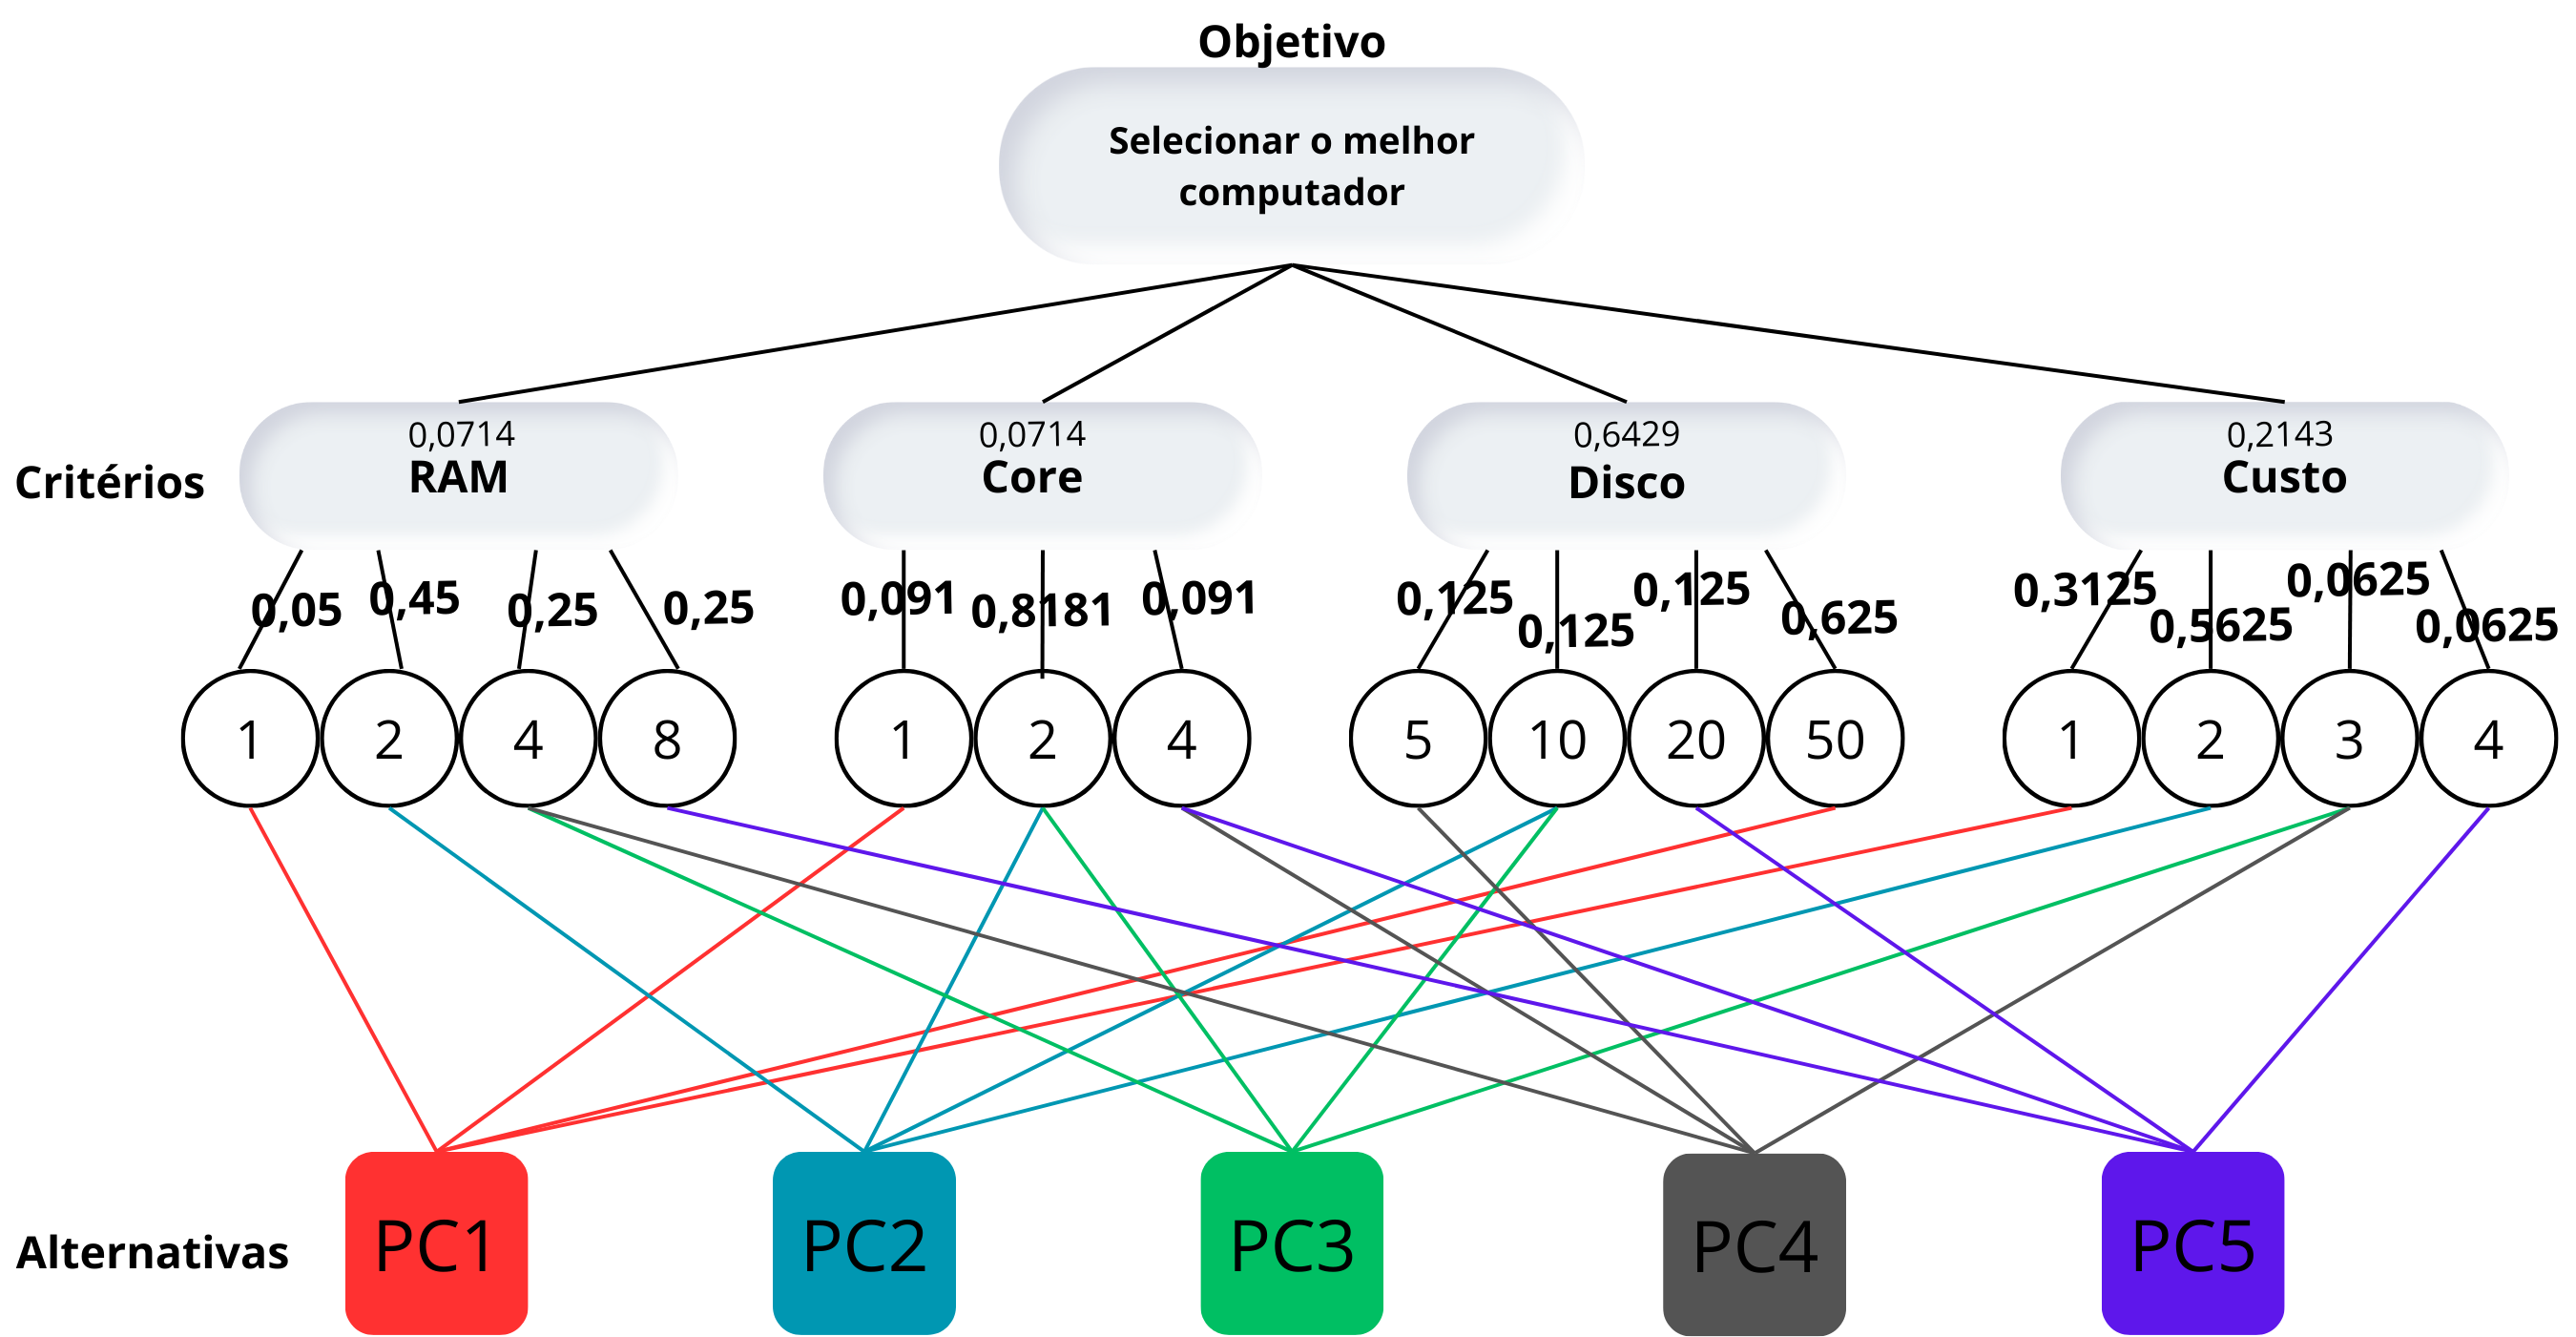
\includegraphics[scale=0.22]{assets/problemFinal.png}
\caption{Tabela matriz de julgamento de RAM}
\label{tab:matJulgRAM}
\end{figure}

Ao final o algoritmo faz mais dois passos, o primeiro é calcular a pontuação de cada alternativa com base nos pesos dos valores de cada critério (figura \ref{tab:pts}) que a alternativa contem, e o passo final é apresentar as melhores alternativas (tabela \ref{tab:rank}), ou seja, o ranqueamento das alternativas com os melhores pontuações.

\newpage
\begin{table}[ht]
\centering
\begin{adjustbox}{width=1\textwidth}
\small
\begin{tabular}{|c|l|c|}
   \hline
   Alternativas  & Calculo & Ponto \\
   \hline
   PC1  &  0,05*0,0714 + 0,091*0,0714 + 0,625*0,6429 + 0,3125*0,2143 & 0,4788 \\
   PC2  & 0,45*0,0714 + 0,8181*0,0714 + 0,125*0,6429 + 0,5625*0,2143 & 0,2914\\
   PC3 & 0,25*0,0714 + 0,8181*0,0714 + 0,125*0,6429 + 0,0625*0,2143 & 0,17 \\
   PC4 & 0,25*0,0714 + 0,091*0,0714 + 0,125*0,6429 + 0,0625*0,2143 & 0,1181 \\
   PC5 & 0,25*0,0714 + 0,091*0,0714 + 0,125*0,6429 + 0,0625*0,2143 & 0,1181 \\
   \hline
\end{tabular}
\end{adjustbox}
\caption{Calculo dos pontos das alternativas}
\label{tab:pts}
\end{table} 

\newpage
\begin{table}[ht]
\centering
\begin{adjustbox}{width=0.5\textwidth}
\small
\begin{tabular}{|c|c|}
   \hline
   Rank & Alternativas \\
   \hline
   1º & PC1  \\
   2º & PC2  \\
   3º & PC3 \\
   4º & PC4  \\
   5º & PC5  \\
   \hline
\end{tabular}
\end{adjustbox}
\caption{Ranqueamento das alternativas}
\label{tab:rank}
\end{table} 

\subsubsection{Cálculo do algoritmo Biblioteca}

\section{APRESENTAÇÃO E ANALISE DOS DADOS}
\section{CONCLUSÕES FINAIS}

\newpage
\bibliography{refs}
\end{document}

